\hypertarget{Systemsekvensdiagram}{}
\section{Systemsekvensdiagram}
Systemsekvensdiagrammet viser hvordan Gem Api use cases fungerer i praksis, og hvordan de forskellige lag i vores applikation fungerer.
\\
Vi har valgt at dele det op i frontend og backend, der gør det nemmere at overskue det konkrete opdeling af de to ting.
\\\\
Gem Api går i alt sin enkelhed ud på at brugeren indtaster noget data og forsøger at gemme det i databasen.
Hvis dette ikke lykkedes, får brugeren en fejlbesked. Nedenfor er denne sekvens visualiseret.
\begin{figure}[H]
    \makebox[\textwidth]{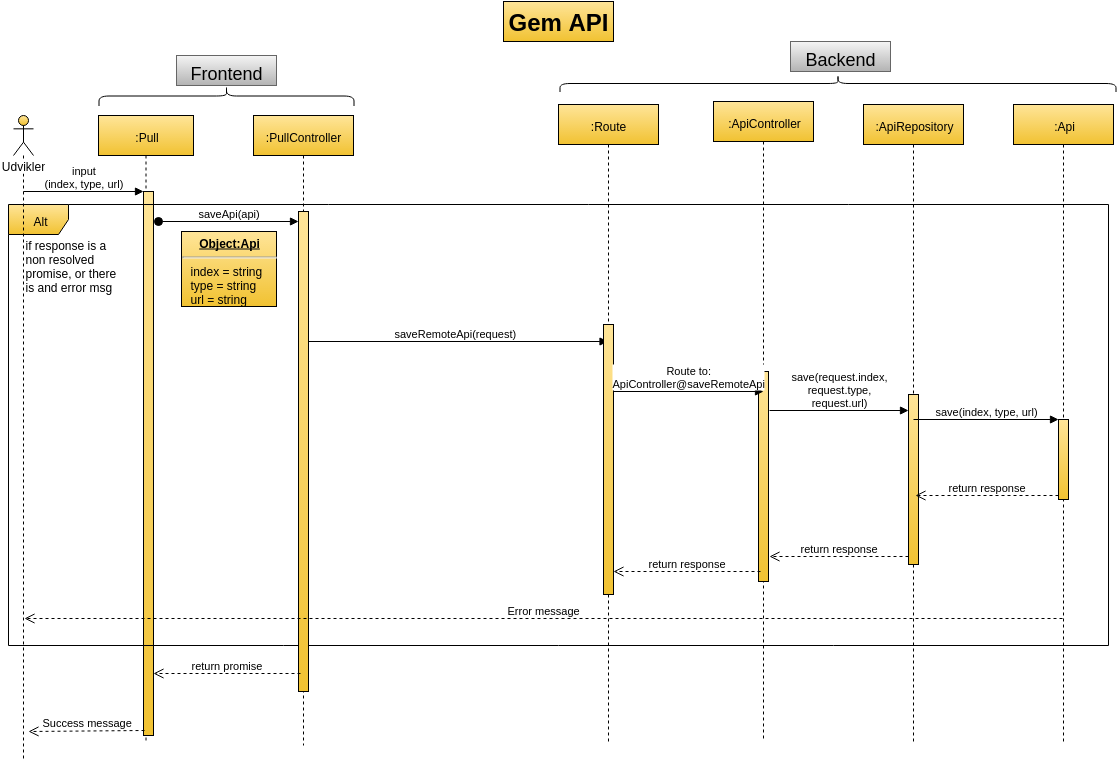
\includegraphics[scale=0.50]{Systemsekvensdiagram}}
    \caption{Systemsekvensdiagram for Gem Api}
\label{fig:ssd}
\end{figure}
